\section{Implementation}

The client and server applications were functionally structured as two separate projects, each version controlled with \textsf{git} and hosted online with GitHub.  

\subsection{Client}

Following previous discussion, the choice of a mobile app still left the question of the exact implementation. Because I would be using \textsf{MapKit}, a native iOS application was a natural fit. The app was coded in Swift, a programming language developed by Apple explicitly for native application development on Apple hardware. This was paired with \textsf{SwiftUI}, a new framework also developed by Apple for building user interfaces. Swift and \textsf{SwiftUI} have, respectively, the benefit of interoperability with Objective-C, Apple's earlier programming language, and existing Apple interface frameworks like \textsf{UIKit}.

\textsf{SwiftUI} is a declarative framework, meaning that the user interface is simply described by the developer. This description is then translated by \textsf{SwiftUI}'s layout engine at compile-time~\cite{apple_2022}. As a result, most of the presentation logic is actually handled by the framework itself.

\subsubsection{Interface Design}

Before any code could be written, however, it was necessary to determine the general design of the user interface and the desired user flow. I wireframed the user interface using \textsf{Excalidraw}, a free and open-source tool for diagram sketches. Each screen in the wireframe was then ultimately translated into a \textsf{SwiftUI} view. \cref{fig:screenshot} demonstrates the final appearance of the app after implementation.

\begin{figure}
    \centering
    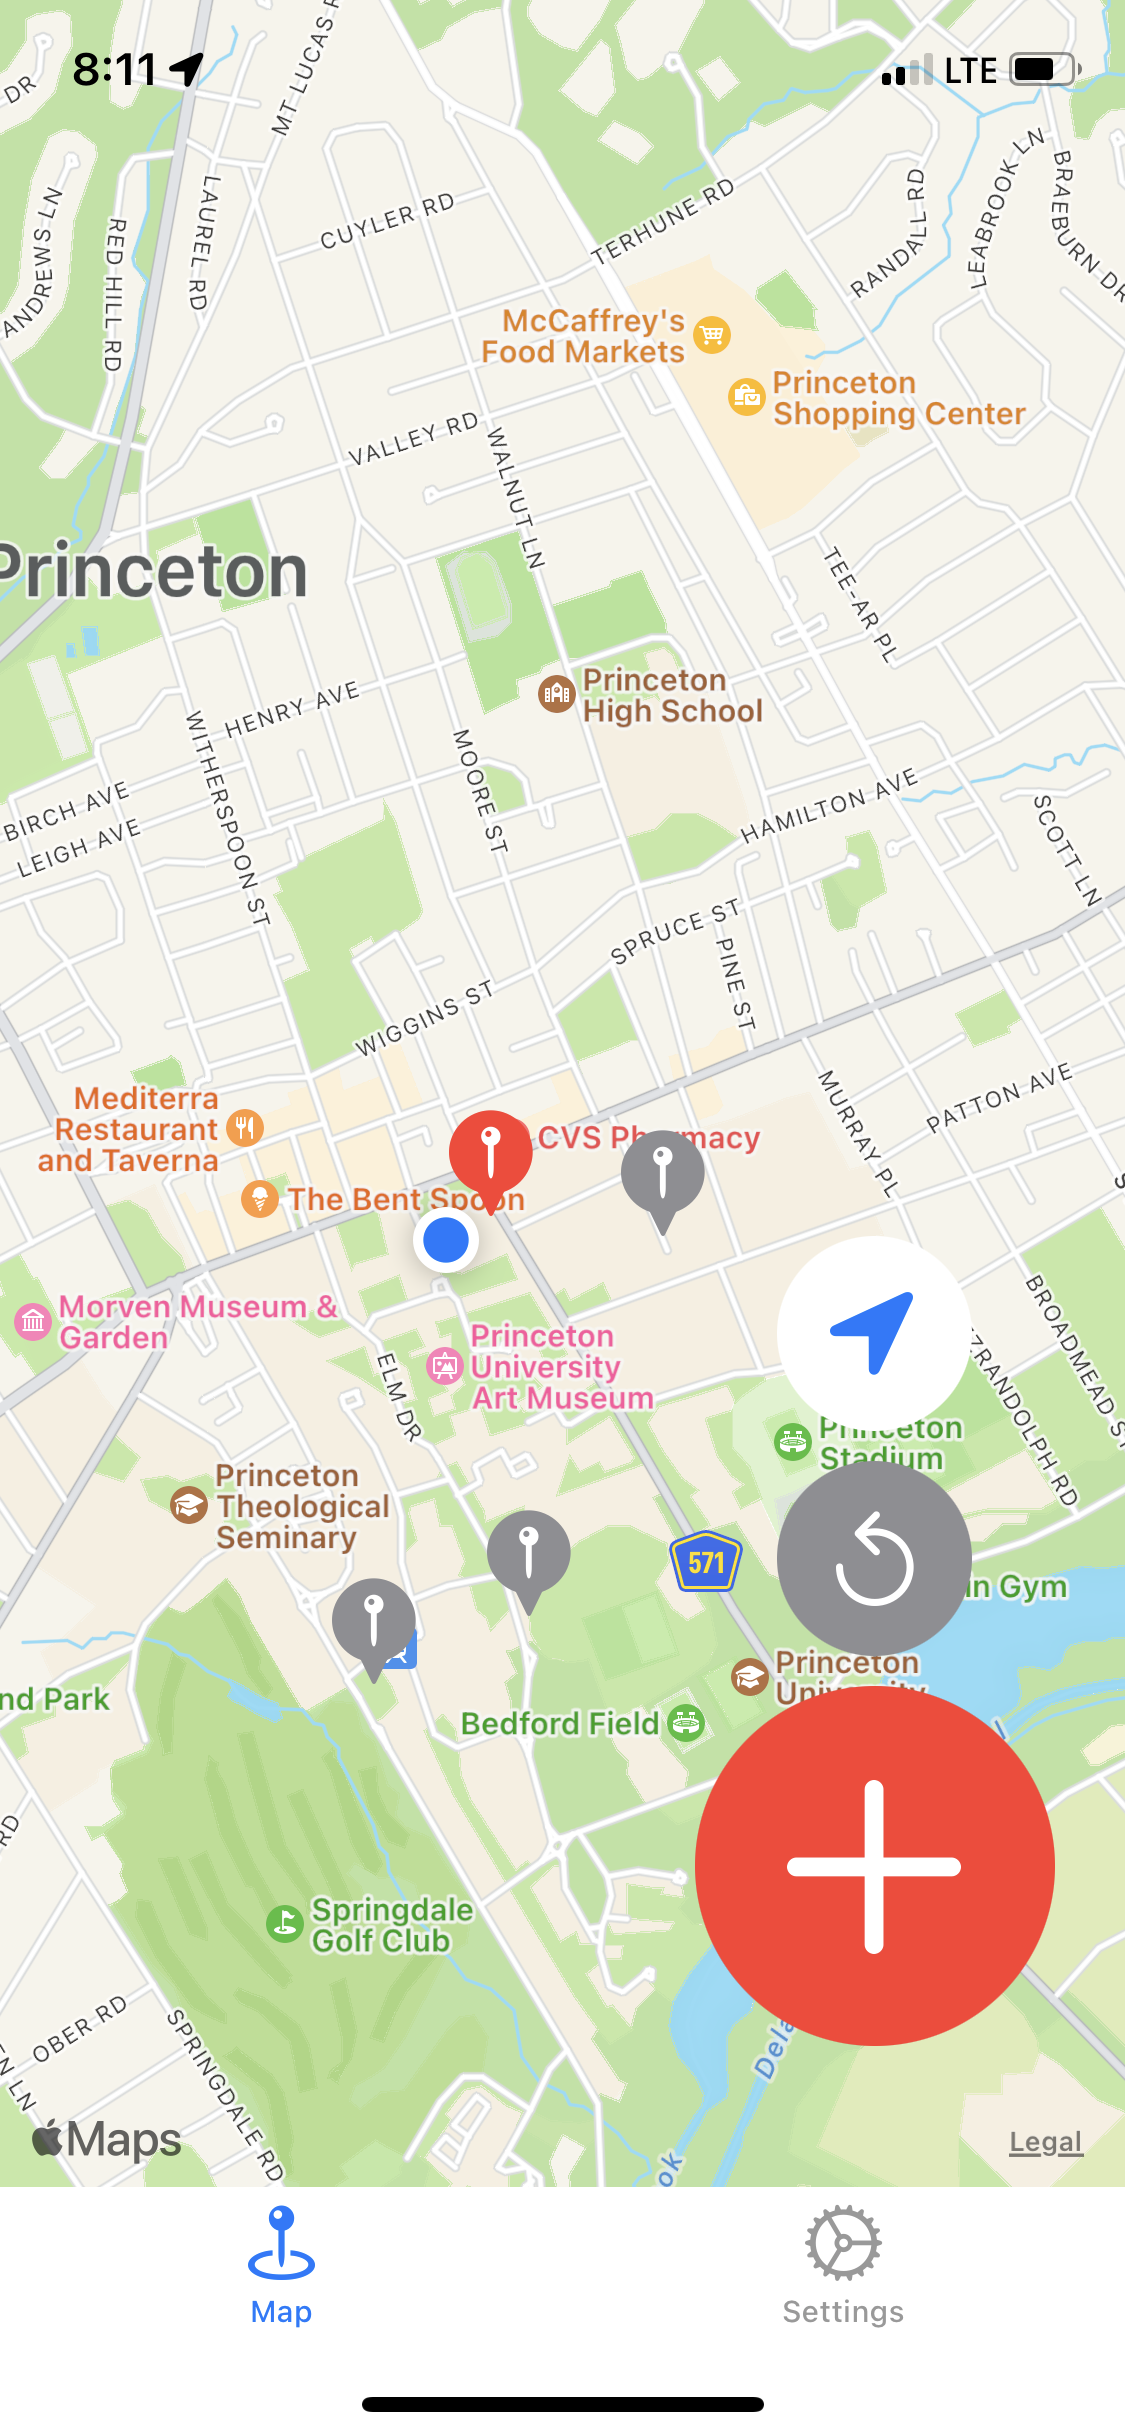
\includegraphics[width=0.5\linewidth]{screenshot.png}
    \caption{Screenshot of the main map screen}
    \label{fig:screenshot}
\end{figure}

\subsubsection{Application Architecture}

The use of \textsf{SwiftUI} naturally separates layout and appearance from the actual business logic of an app. From this, I chose the Model-View-ViewModel (\textsc{MVVM}) pattern as the underlying architecture. \textsc{MVVM} decouples presentation logic (\emph{views}) from business logic (\emph{models}) by using intermediate objects called \emph{view models}. The state of each view is bound to the associated view model, which facilitates interaction with models and user input~\cite{britch_2021,hudson_2019}.

Each part of the final user interface is composed of one or more \textsf{SwiftUI} views, with view models being used as necessary to handle state management and any dynamic behavior. In any application, it is likely certain logic needs to be shared throughout the overall system. My app needed to access global settings, authentication state, and location services at multiple points. To solve this problem, I wrote different \emph{managers} that represented a shared service layer. When required, these managers were injected into a view model to access the appropriate services.

\subsection{Server}

Compared to the client app, the server required drastically fewer lines of code. However, the difficulty was in composing the separate technologies that made up the server's basic functionality. The core \textsc{API} is handled by \textsf{FastAPI}, a high-performance web framework written in Python. I chose Redis, an in-memory datastore, as the database for its ease-of-use and included geospatial capabilities.

These core services are packaged together as one Docker application. Docker is used to containerize the server, which isolates the app from its environment. By using Docker, I could develop, test, and deploy the server on different machines while ensuring that each build would behave the same.

\subsection{Deployment}

In order to distribute the client app to users, I relied on Apple's TestFlight service. TestFlight allows developers to beta-test their iOS applications and receive feedback from users. The benefit of this approach was that I did not have to go through the full App Store approval process in order to deliver my app to testers.

The server was deployed on a DigitalOcean Droplet. Each Droplet is a Linux virtual machine (\textsc{VM}) that runs on virtualized hardware. After reserving an instance, I could access the Droplet remotely using \textsc{SSH} and install all required code and tools using \textsf{git} and the system package manager.
